\section{Electrical Energy Storage}
\label{ch-introduction:sec:energy-storage}

The idea of using energy storage in the electricity grid has been discussed for quite some time, and its important role in future energy systems has already been identified in the 70s \cite{Kalhammer1979}.
As the name suggests, electrical energy storage systems have the ability to both consume, store, and release electrical energy by converting it into a different form of energy.
Depending on the rate at which energy can be consumed and released, i.e. the system's power, as well as the amount of energy that can be stored, i.e. system's capacity, different functions can be provided.
A study for the Department Of Energy (DOE) showed that, when correctly exploited, these functions can yield direct financial benefits of \$157.56 billion over an estimated 10 year system lifecycle \cite{Eyer2010a}.
Figure \ref{ch-introduction:fig:storage-financial-benefits} shows these benefits in relation to their typical discharge period, and links them to their associated functions, too.
Here, Time Of Use (TOU) energy cost management yields the largest economic profit, yet from a historical point of view, bulk energy storage has played the most important role in the energy system.
This kind of storage was used for large scale time-shifting and allowed the balancing of demand and supply without the need of ramping up or shutting down conventional power plants.
Nowadays, this kind of storage can also tap into emerging revenue streams, i.e. to relief network congestion, thus deferring the need for network reinforcement whilst allowing the integration of volatile renewable energy sources.
So far, 127GW of bulk energy storage has been built worldwide \cite{Rehman2015}, tripling it ever since Kalhammer's publication \cite{Barbour2015, Barbour2016}.

\begin{figure}\centering
	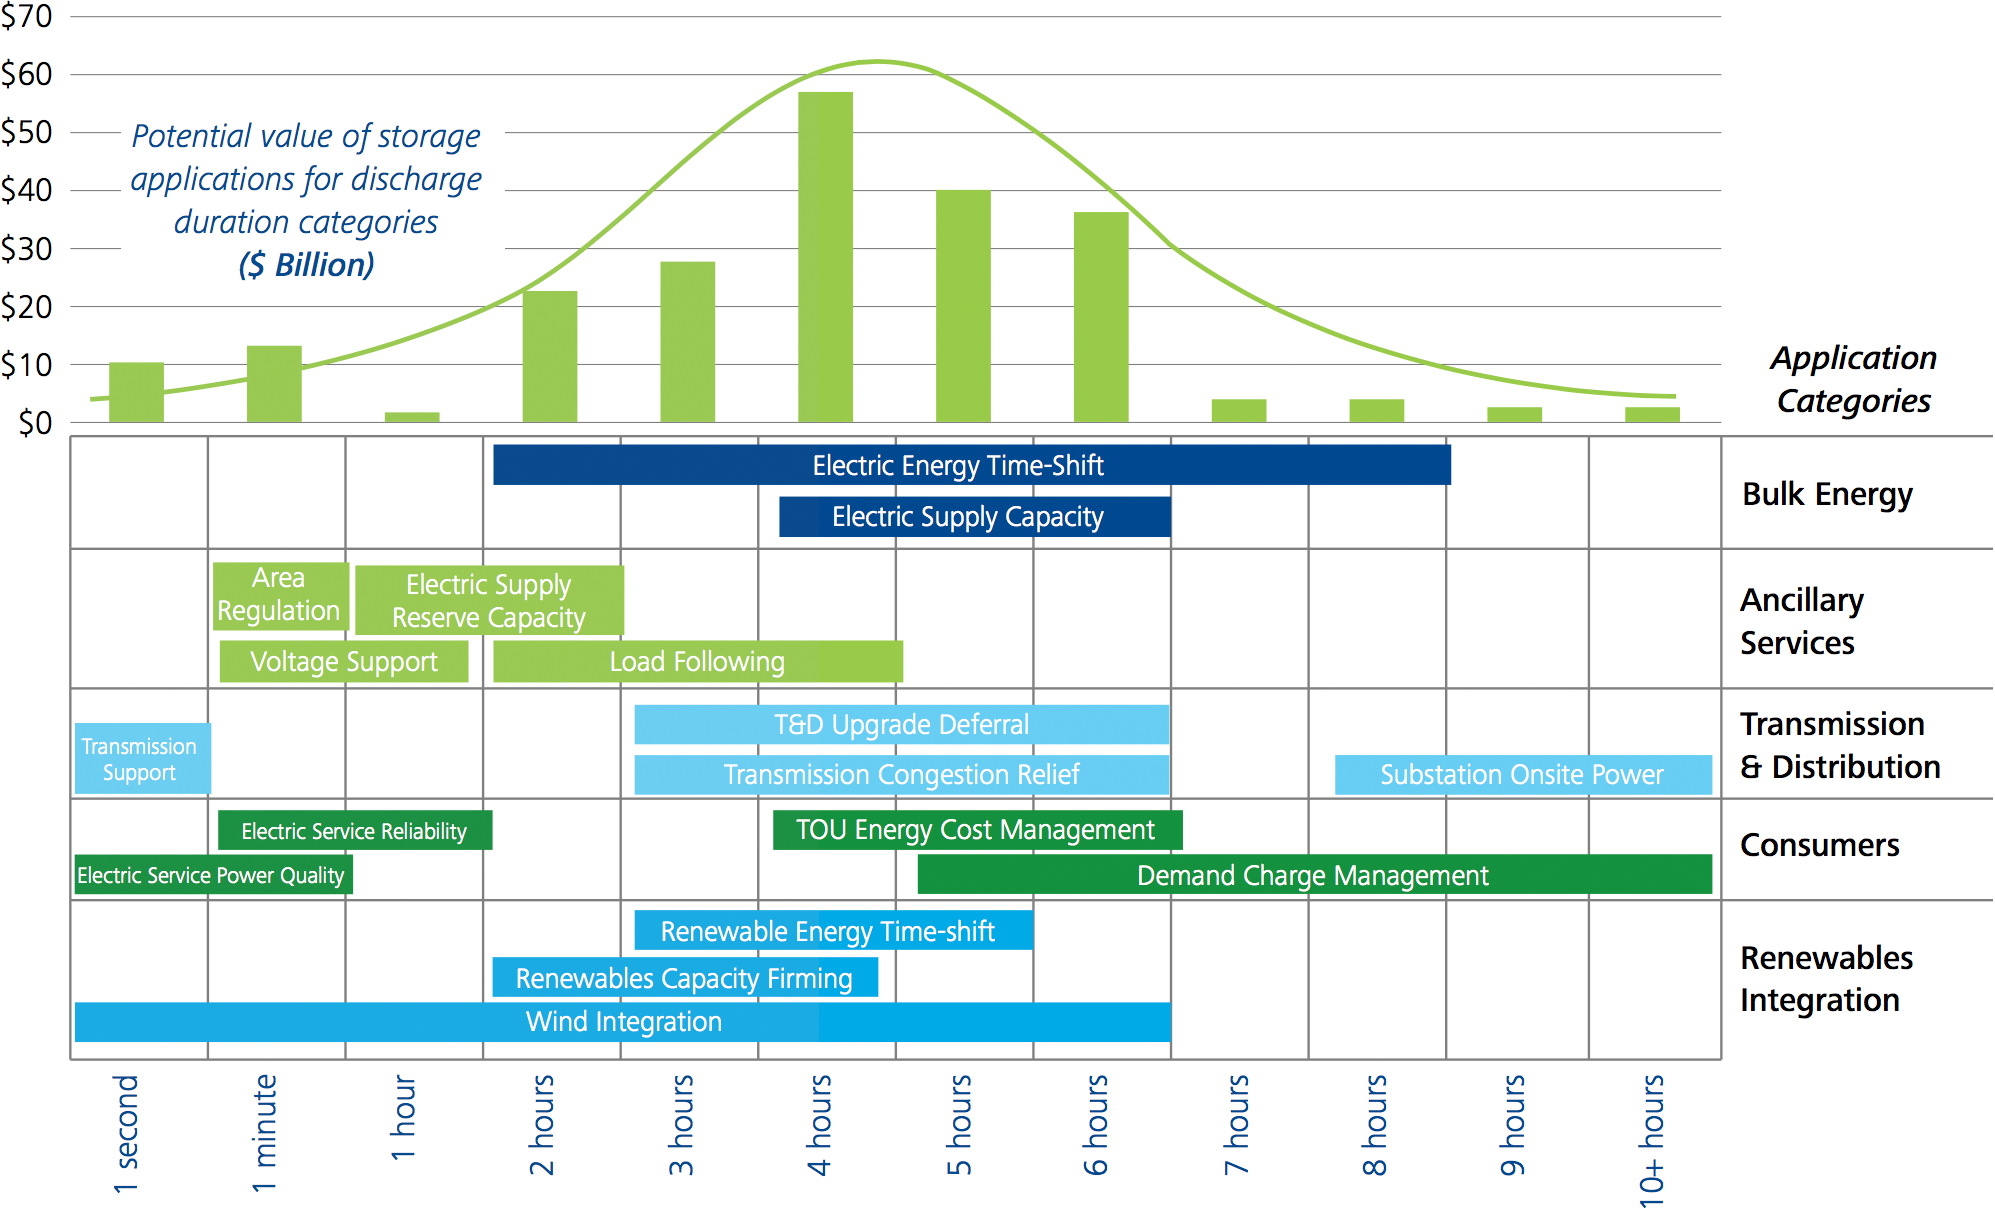
\includegraphics[width=\textwidth]{_introduction/fig/storage-financial-benefits}
	\caption{Energy storage applications and corresponding value for various discharge durations \cite{Deloitte2016}}
	\label{ch-introduction:fig:storage-financial-benefits}
\end{figure}

However, the scale and lack of responsiveness of such bulk energy storage systems prevents them from being used in local distribution networks where fast system responses are required.
Different energy storage technologies and their applications are briefly introduced in this section.

\subsection{Energy Storage Technologies}

The oldest form of grid scale energy storage, i.e. for bulk energy storage, is pumped hydro-electric energy storage.
In 2012, 99\% of bulk storage was comprised of pumped hydro \cite{TheEconomist2012a}.
Since pumped hydro is not a suitable technology for distribution network implementation, it is not considered in this technology assessment.

One of the first comprehensive reviews that included small- to medium-scale energy storage technologies was published by McLaron and Cairns \cite{McLarnon1989}.
They discussed electrochemical energy storage,
%\footnote[1]{i.e. lead-acid batteries, iron/nickel-oxide batteries, zinc/chlorine batteries, zinc/bromine batteries, redox batteries, hydrogen/nickel oxide batteries, metal/air batteries, sodium/sulfur batteries, sodium/metal chloride batteries, lithium/iron sulfide batteries, and lithium/iron disulfide batteries},
thermal energy storage,
%\footnote[2]{i.e. aquifers, latent-heat storage systems, aqueous systems, salt hydrates, clathrates, molten salt systems, and more},
mechanical energy storage,
%\footnote[3]{pumped hydro-electric energy storage, compressed air energy storage, flywheel energy storage},
chemical energy storage,
%\footnote[4]{hydrogen generation, storage, transmission and utilisation},
and magnetic energy storage.
%\footnote[5]{superconducting magnetic energy storage}.
With subsequent advancements in technology, Battery Energy Storage Systems (BESS), Compressed Air Energy Storage Systems (CAESS) and Flywheel Energy Storage Systems (FESS) have become the most promising choices for deployment in distribution networks \cite{Ibrahim2008, Chen2009, Hadjipaschalis2009}.
However, with no moving parts, the increasing energy density, and improved control systems, batteries are starting to outperform the competition.
They can be deployed in ever decreasing form factors and are about to outlast their competition, too \cite{Luo2015}.
Furthermore, Battery Energy Storage Systems (BESS) can provide a multitude of functions; unlike their competition.

\subsection{Energy Storage Applications}

The traditional utilisation of energy storage was standby reserve.
This use case was particularly compatible with bulk energy storage, since the energy volume of sufficient scale to cater for unanticipated national energy demand \cite{Guney2017}.
Smaller scaled energy storage systems, including BESS, are however capable of providing even faster response.
With more sophisticated control systems, they can provide functions like \cite{Katsanevakis2017}:

\begin{itemize}
	\item energy shifting (or ``arbitrage''),
	\item supply capacity,
	\item ancillary services (e.g. load following, frequency regulation, spinning reserve, non-spinning reserve, supplemental reserve, voltage support, black start)
	\item grid stabilisation (e.g. rotor angle stability, voltage stability, sub-synchronous resonance)
	\item upgrade deferral
	\item service reliability
	\item power quality
	\item renewables integration (i.e. arbitrage, firming, smoothing)
\end{itemize}
















